現代で通信という言葉を聞いた時、連想される多くはインターネットを始めとした様々な電気通信だろう。だが、電気通信ができる以前より、人は様々な意思疎通…通信を行ってきた。本章では、電気通信に至るまでの人の意思疎通の営みを見ていく。これらの営みの中で、人間は通信に必要とされる要件を見出してきた。通信とは何か、何が必要なのか。まずは歴史からその要件を学び取っていこう。

\section{声による伝達}

動物には種によって様々な対話方法がある。蝙蝠なら超音波を使い、鳥ならば鳴き声で対話を行う。動物の鳴き声のモノマネで知られる江戸家小猫氏によれば、人間に最も近いゴリラなどは10種類の鳴き声により様々な対話を行うという。例えば、我々がゴリラの鳴き声と聞く「ウホウホ」という鳴き声は、特に喜ばしい時、幼いゴリラが使うことが多い表現なのだそうだ。我々人間にその差異はなかなかわかりづらいが、しかしながら種ごとの鳴き声による伝達は、我々人間の発話による伝達に同じことなのだという。

\subsection{人間の発話}

自らの声帯により何らかの音を出し、これに意味を持たせて伝達する。我々人間が知る多くの動物の鳴き声にはそれほど多くの種類の伝達はなく、概ね自らの感情の伝達が中心となっているようではあるが、人間の発話による伝達もそれと同様である。生まれてすぐの赤子は、泣くという動作を伴った発話により自身が不快であることを伝える。成長し、感情が分化する(図\ref{fig0_1})につれ、何が不快なのかなどもその泣き方に入ってくるようで、親はその泣き方で状況を察することも少なくない。やがて、言葉を覚え話すようになると、それらの言葉の意味を経験から学ぶようになる。家族から広がるコミュニティの中で、共通した意味の言葉を使うようになり、人との伝達・コミュニケーションを始めていくのである。

\begin{figure}[htbp]
\centering
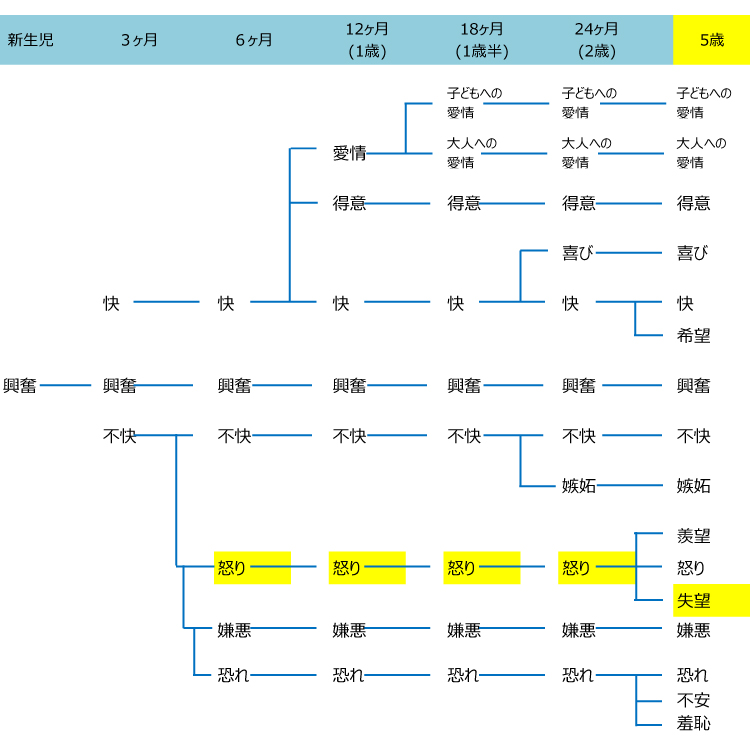
\includegraphics[width=0.6\linewidth,keepaspectratio,bb=0 0 750 750]{fig/fig0_1.jpg}
\caption{ブリッジスの情緒分化図 日本病児保育学会ブログ記事より引用}\label{fig0_1}
\end{figure}

コミュニティの違いによる差異こそあるものの、我々人間の"鳴き声"は言語を為し、その共通認識により対話、伝達が始まったのである。この言語は感情にとどまらず、具象抽象の垣根を超えて叙事や論証、または歌や言葉遊びと言った様々な知的活動の礎となった。動物の鳴き声による対話と対応した人間の会話は、最も原始的な伝達の方法であるものの、様々に技術が発達した今なおコミュニケーションの基礎を為している。通信の始まりは、このような"発話による伝達"であったといえよう。

\subsection{発話の制約}
しかし、単純な発声による発話では、声が届く範囲にしかその意味が届かない。この時の届く範囲とは、空間的な範囲もあれば時間的な範囲でもある。落語会が行われていた会場に、終わった後に入っても落語を聞くことはできないし、また、同じ時間に遠く離れた場所にいても落語を聞くことはできない。肉声の落語を聞くことができるのは、その時その場所で演者と同じ空気を共有していた者に限られる。逆に、その空気を共有している者の中では、選択的に伝えたり聞いたりするということも難しい。高座の上で演者が下座に何らかの指示を出す時、声を使うとすれば客席の幾人かにはどうしても聞こえてしまう。同じ会場で鼾をかいて眠る客がいたとして、これだけを聞かないというのもなかなか無理がある。

先の鼾の例のような雑音があった場合などは特にそうだが、発話によるコミュニケーションでは聞き取れない・追いつかないと言った問題も発生する。マンツーマンのゆっくりした対話であれば言い直してもらえばすむだけの話であるが、先の落語のような例では、そういうわけにも行かない。音自体が聞こえなかった、音は聞こえたけれども判別がつかなかったと言ったレベルから、言語的な問題…イントネーションの差異、語彙にない単語の使用、そもそも言語が異なる、勘違い…と言った知識や思考の問題まで、発話の時には伝達の誤りが起こりうる。

発話による伝達は、原始的であるがゆえに手軽ではあれど制約や問題も内包している。通信・伝達技術というのは、これらの制約や問題を如何に打破するのかという人間の飽くなき挑戦の成果であるとも言える。

\subsection{口伝という方法}
発話の制約を最も単純に外したのは\textbf{口伝}\index{くでん@口伝}である。現在でも民話や民謡など、様々なものが口伝により伝えられているが、これは人間の記憶を介することによって時間や空間の制約を緩和したものといえよう。最も身近なところでは、伝言がそうであろう。もっとも、伝言ゲームに見られる通り、伝達の誤りという問題は解決されているとは言いがたい。「JPCZによる擾乱の影響で山陰地方を中心に荒天となる」などと専門の用語が入った言を伝言したところで、途中に知らぬ人が入れば伝言がうまく行く可能性は低いだろう。また、伝言には意識的・無意識的な取捨選択もあり、伝達の誤りという観点ではむしろ増えているかもしれない。

しかしながら、人間以外の資源が必要ないこの口伝という方法は、最も初期から存在すると同時に、現代まで続いている伝達方法である。口伝の国内における最も古い例としては、稗田阿礼が挙げられる。古事記には彼(彼女?)の誦により伝えられたものが筆録されている。その後の歴史にも、説法や講釈と言った例はほぼ口伝であったようだ。一方、現代で行われている口伝の例としては、先にも持ちだした落語を例に挙げたい。昭和の爆笑王、桂枝雀師は著書「枝雀とヨメはんと七人の弟子」の中で次のように書いておられる。

"一番最初は「ちょっとやるから聞いてなさい」と言って、一字一句口移しで教えることから出発いたします。やらせてみて、ちょっと違うとイントネーションから直す。それが段々お稽古やっていくうちに、五分なら五分、流れを教えるようになる。"

これは、平成のはじめ頃に書かれた文であるし、枝雀師は99年にお隠れになったから、いま他の噺家が同様のやり方をしていると言い切ることはできない。だが、筆者が、この枝雀師の三番弟子、文之助師に"つる"を教わった時は、ほとんどこの通りの教え方であった。ただ、カルチャースクールでのことであるから、録音し、自分で原稿に起こし、その上で直してもらいながらという指導であった。とはいえ、これも口伝には違いない。多くの伝達法がある中で、わざわざこの原始的な口伝という方法で伝承をするのはなぜだろうか。

それは、口伝によってしか伝えられない、空気や情感、発生、身振り手振りの細かな違いなどを伝えられるというところであろう。現代の技術をもってすれば、双方向で似たような指導を遠隔地間で行うことも可能であるように見える。しかし、それでも微妙な空気感や息の間といったものは伝えきれない。落語という芸能は高座の落語家と客席が一体となって作り上げる空間が生命であるから、なるほど、その部分を伝えるためには口伝を取るよりほかないのであろう。また、落語は時代により変化していくものであるから、口伝という形態での変化は逆に追い風となるのであろう。これは、落語の伝承が「ネタの原稿を伝える」のみでないことを示しているといえる。

現代の視点からすれば口伝は古臭く、非効率な手法に見えることも多い。だが、それを意図して取り込んでいる芸に学べる通り、口伝でこそ伝わることもある。通信・伝達技術の多くは、重要と考えにくいものや伝えづらいものを取捨選択しているのである。逆に、その捨てられたものを拾う価値があるシーンや、そこまでの効率を要求しないシーンがあるからこそ、一見古臭く見える通信・伝達の方法も現代に息づいているのである。


\section{筆写による記録}

口伝は人間の記憶を媒介にして時間や空間の制約を打ち破った。しかしながら、当然全ての人間が稗田阿礼のような記憶力を持つはずもないし、伝達も記憶も個人の状況に依存することとなる。これを打破するのは日本へと輸入された文字、そして筆記媒体であった。

\subsection{文字と図画}

文字とそれを記録する媒体は、ヒエログリフやパピルスと言った著名な例があるとおり古代エジプト文明の時代にまで遡る。楔形文字や漢字と言った様々な文字が青銅器時代に生まれたのである。日本へ文字が入ってくるのは弥生時代とされ、それからの後、8世紀頃には先の稗田阿礼の言を元にした古事記(図\ref{fig0_2})や風土記、日本書紀といった書物が発行された。

\begin{figure}[htbp]
\centering
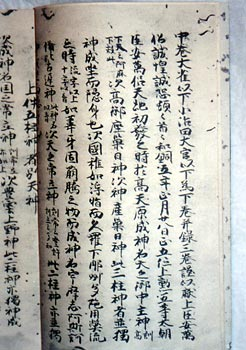
\includegraphics[width=0.6\linewidth,keepaspectratio,bb=0 0 246 350]{fig/fig0_2.jpg}
\caption{真福寺収蔵の国宝・『古事記』 Wikipediaより引用}\label{fig0_2}
\end{figure}

文字の輸入に伴い、離れた場所に文字を書いた媒体を送るという形式での伝送も行われるようになっていった。それらの書物の中には何百年という時を経てなお現代で読むことができるものも多い。これは、文字とその記録媒体が時間と空間の制約を打ち破ったということである。著名な数学者の書簡や日記が見つかることもあれば、伝わるつもり無く詠まれた"この世をば 我が世とぞ思う 望月の 欠けたることも なしと思えば"が現代にまで伝わっている(道長本人は記録に残さなかったが、その場に居合わせた人が日記に記したために現代まで伝わっている)など、文字は言語によって表現可能なものの時間的・空間的制約を打ち破ったのである。汚損や焼失といったリスクこそあるものの、口伝や発話の段階からすれば大きく進歩したと言えるのは明らかであろう。

また、これらの媒体は図画の伝達も可能とした。これは、発話や口伝で伝えられなかったものを伝えられるという利点をもたらした。紙媒体は、文字を媒介に発話を記録すると共に、図画として描けるものも記録する媒体なのである。

\subsection{写本から複写へ}
主として紙媒体に記述された文字による通信は、複写されて更に伝えられることにより、口伝やうわさ話と同様に広く伝わる手段となった。写本はその最も原始的な例である。紀元前3世紀、アレクサンドリア図書館では既に組織的な写本が行われていたとされる。別には、ギルガメシュ叙事詩もその頃の写本を最初とし、原本こそわからぬものの現代まで継がれている。日本においても多くの写本がある。特に源氏物語などは、既に写本が遠距離の伝達の役割を担っていたことが、菅原孝標女が更級日記に記述した例などからわかる。

先に述べたとおり、筆記にまつわる媒体には確かに汚損や焼失というリスクがある。これ以外にも、数十年・数百年という時の流れの中で退色するようなものもあれば(現代に流通しているボールペンインクの多くや、万年筆のインクなどは必ずしも長期保存に適するものばかりではない)、言語や文字が滅びて内容を理解できないというものもある。しかし、複写による流通は、これらのリスク解決に対し、"冗長性"という解決策を与えた。つまり、写本の1冊が残れば伝わる緒は紡ぐことができ、翻訳により別言語へと訳されていれば滅びた言語を用いずとも内容を理解することができる。

現代においてバックアップと呼ばれる手法も、原理としては複写と同等である。その観点から言えば、複写は多方向への同時期の通信・流通を可能にしたのみならず、その安全性において起源的なものといえる。紙と図画・文字による伝達は、複写によって通信の時間的・空間的制約を打ち破るとともにその冗長性などを(意識的かどうかは不明ではあるが)確保したのである。

無論、人間の手による複写は手間であるし、また誤りもある。そのため、短時間で多くの複写を行う印刷技術が発達した。8世紀には既に木版印刷の技術が生まれていたようで、その後も活版(凸版)印刷、銅版(凹版)印刷、平版印刷と多くの印刷技術が追随していくこととなる。広い意味では、印鑑などもその一例とも言え、承認の意を当人しか原版を持たない複写によって表しているとも考えられる。このように、複写・印刷の技術は、通信の幅を大きく広げた、その代表的なものと言える。

\subsection{筆記媒体が捨てたもの}
一方、筆記媒体・印刷媒体は視覚によって通信できないものを取捨選択している。音や匂い、手触りや味といったものを、筆記媒体・印刷媒体のみで完全に送ることは出来ない。勿論、これらが必ずしも必要だとは限らない。ただ、筆記媒体は、図画と言語によって伝えられるもののみを選択し、結果として他を捨てることで、通信に様々なメリットを生み出したのである。

具体的な例を見てみよう。先に、ゴリラには10種の鳴き声があると書いた。これらの鳴き声を、我々は正確に伝わるように書き分けられるだろうか。あるいは、その各々の声のシチュエーションを解説するとき、十二分な語彙・表現があると言い切れるだろうか。おそらく、この問にYesと答えられる人は少数であろう。では、この鳴き声の差異が現実に必要となるような例はあるだろうか?その道の専門家でもない限り、これを文字で正確に伝えなければ困るというケースは考えにくい。十分な語彙・表現と図画を以って伝達するとき、筆記媒体が捨てた要素は確かに存在するのであるが、一方でその要素が必要なケースでなければ、筆記媒体による通信によりその利便性のみを享受できるのである。



\section{遠距離の高速通信}

筆記媒体によって破られた制約は多いが、しかし、筆記媒体にも難点があった。通じるのに時間がかかるという点である。

\subsection{持ち運ぶことの難点}

郵便碁という遊びを考える。現代において、遠く離れた場所にいる二人が囲碁を打ちたいとすれば、インターネット上のゲームサイトにアクセスするなどすれば、ほぼリアルタイムで遊ぶことができる。しかし、それがなかった明治の頃、ハガキに一手ずつ手を書いて送る"郵便碁"が生まれた。現代の郵便制度を持ってしても、1局に1年から2年はかかる。通常は一度に4つの手を送り、4局同時に進めたそうであるが、それでも非常に多くの時間がかかる。日本郵便碁愛好会に所属されているようなじっくり楽しみたい方はともかくとして、遠方の友人と会話がてら軽く打ちたいという時に気軽に楽しめるとは言いづらい。

郵便制度の発達の前には伝書鳩や飛脚により同様の伝達が行われていた。しかし、時間がかかるという点はいずれも変わらないようである。明石飛脚という噺では足に自身のある男が大阪から明石までの約15里(現代で言うと約59km相当)の道のりを一日かけて片道だったという。無論、交通手段が未発達であったという時代背景もあろうが、現代でも郵便は大抵遅い手段として知られる\footnote{これは非常に特殊な例であるが、10TB容量のHDD400台を詰めた箱を2日かけて車などで運べば、185Gbpsという驚異的な速度になる。読み書きの時間は無視しているし、それだけ大容量のデータを運ぶ必要もないだろうが、データ量が著しく多い場合は郵便が最速になることも考えられる例としてここに記した。}。

\subsection{視覚による通信}

マラトンの戦いの例がもっとも古いものとして知られるが、戦況を知らせるような伝令は内容こそ多くなくとも速度が要求される。そこで、視覚的に伝えられるものに何らかの意味を定めておき、遠距離でも素早く通じるようにした。狼煙や手旗信号(図\ref{0_4})がそれである。現代でも、野球でベンチから監督が出すサインはこれに当たるだろう。また、筆記媒体も介していることとなるが、アドバルーンもその一例と言える。

これら視覚による通信は視線を確保することが要求されるが、通常人間が見える範囲においてはタイムラグなしに通信を行うことができる。また、中継も比較的容易い。手旗信号や筆記媒体など、細部を見る必要がある手段だと距離こそ短くなるものの、伝達にかかる速度自体は高速で、音では届かない距離でも伝達できることには変わりない。一方、その意味付けの少なさから、多くの情報を伝えるには不向きである。

\begin{figure}[p]
\centering
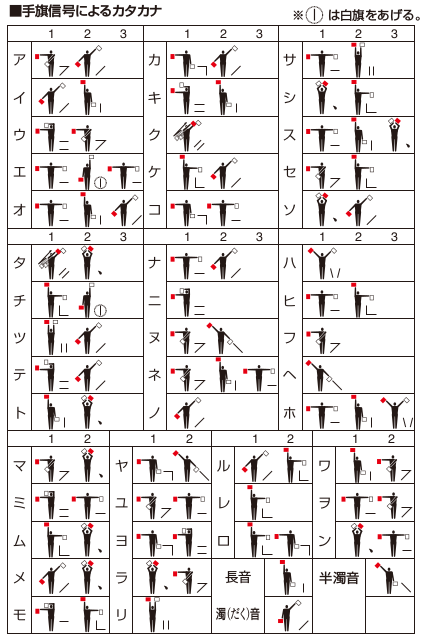
\includegraphics[width=\linewidth,keepaspectratio,bb=0 0 424 637]{fig/fig0_4.png}
\caption{カタカナの手旗信号 海上自衛隊・海の手帳より引用}\label{fig0_4}
\end{figure}


\subsection{視覚の通信が捨てたもの}

視覚による通信は、速度を重視したがために、伝えられるものが非常に限定的なものとなった。手旗信号や狼煙であれば、前もって決められた意味付けの範疇に属するものしか伝えられないのである。また、狼煙は多くの場合一方向的でもあった。逆に、双方向的にも可能な手旗信号は、音やものに比べ受信者が気づきづらいか、あるいは受信者を常にさく必要があった。

インターネット技術の標準化を推進する任意団体\textbf{IETF}\index{IETF}(Internet Engineering Task Force)\index{Internet Engineering Task Force|see{IETF}}は、その標準技術仕様等をRFC\index{RFC}(Request For Comments)\index{Request For Comments|see{RFC}}という形で公開しているが、この中のRFC4824では、手旗信号を用いたIPデータグラムの転送を記している。これは\textbf{ジョークRFC}\index{じょうくRFC@ジョークRFC}として出された仕様ではあるが、手旗信号について(電気通信を元に)実に愉快な考察がなされている。以下、例を挙げてみよう。
\begin{itemize}
\item 送信・受信に各1名以上ずつの、2名以上の組によりひとつのインターフェイス(送受信設備:この場合は人)がなされる。
\item 通信速度は送受信者の経験に依存する。
\item なりすまし防止の為の自己紹介が推奨される。
\item タイムアウト、通信が時間切れとなる感覚はデフォルトで60秒で、手を休めることができる程度になっている。
\item 転送量が多く長時間の通信となる場合は代替のインターフェイスを用意する必要がある。
\item 時間とともに転送速度(帯域幅)が変わり、概ね減少していく傾向にある。
\item リンク内に別のインターフェイスがあった場合受信できるため、セキュリティ的に安全ではない。
\item インターフェイスが送受信したデータを記憶する必要があり、生存時間が定まっていない。
\item インターフェイスを通過したデータであっても、その記憶に残っていることがある。
\end{itemize}
これらの点は、現代の電気通信からすればその多くが特異なものであり、実用上はほぼデメリットと捉えられるものであろう。換言すれば、これほどまでに多くのものを犠牲にしてでも、何よりも速度が必要になる時、初めて手旗信号など視覚の通信に頼る必要が出てくるのである。


\section{通信の秘匿}

先に書いた藤原道長の歌は、本人の意図によらず後世へと伝わったものである。この歌であれば(元々が酒席等の話であったようなので)笑い話で済むが、意図しないところに伝わるのは望ましくないことも多い。対面の方法であれば、本人であることを認識するか、あるいは初対面であれば本人確認をするなどの方法で当人同士とし、他に誰もいない場所で(音漏れがなく、盗聴器なども仕掛けられていない前提であるが)話すなどの方法がある。だが、遠距離の場合、送受信者双方の目から離れる時間が必ず存在する。その時に、秘密を守るため、やはり様々な手法が用いられてきた。

\subsection{未開封証明}

中世のヨーロッパで主に用いられていた方法が未開封証明、封蝋(シーリングワックス,図\ref{fig0_3})である。蝋を垂らし、多くの場合は家紋などを象った、当人オリジナルの封印を施して郵送した。洋形封筒の場合、このシーリングワックスを破損することなく開封して再度元のとおりに戻すのは至難の業である。したがって、全きシーリングワックスの未開封の書状が届くことは、途中で第三者に読まれあるいは改ざんされていないことの証明となった。

\begin{figure}[htbp]
\centering
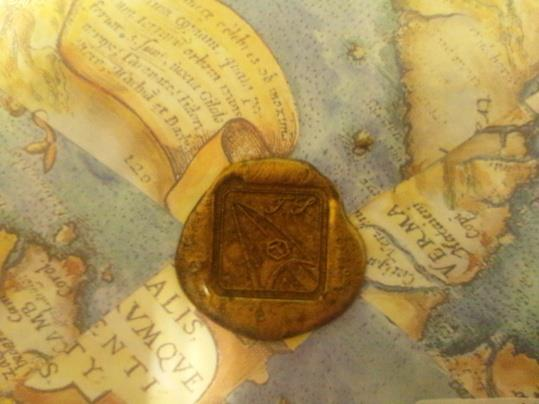
\includegraphics[width=0.5\linewidth,keepaspectratio,bb=0 0 539 404]{fig/fig0_3.jpg}
\caption{筆者の封蝋の例}\label{fig0_3}
\end{figure}

だが、これはあくまでも手紙が届いた場合の話にしか過ぎない。その内容を読むことを目的とする場合、書状を手に入れてしまえば内容は平文であるため、易々と読むことができる。本来の受信者に渡す必要さえなければ、そのまま内々に破棄してしまうことで受信者には何もわからない。これは、現代の郵便制度でも同様であり、心ない郵便局員が一般郵便を持ち帰り、内容を読んだり届けなかったりしたという事件もあった\footnote{少なくとも日本においてはこれが事件として報道される程度に珍しいことであるので、郵便が信用ならないと言っているのではない。寧ろ日本の郵便送達率は9割を超え、世界に冠たる信頼の郵便制度と自負すべきところである。}。

\subsection{暗号化}

そこで、途中で奪われたり盗聴されたりしてもその内容を把握できないよう、\textbf{暗号}\index{あんごう@暗号}が用いられるようになった。

古来の暗号として特に有名なのは\textbf{シーザー暗号}\index{しーざーあんごう@シーザー暗号}である。古代ローマの軍人、ガイウス・ユリウス・カエサル(英語読みでジュリアス・シーザーとなるため、これにちなんでシーザー暗号と呼ぶ)は自身が秘匿としたい文を送るとき、それぞれの文字を"シフト"して送信したという。例えば、aをcに、dをfに、xをzに、yをaに、zをbにと、それぞれ(サイクリックに見て)2文字後のアルファベットへと変えて送信したのである。この規則を知らない(また気づかない)者には、内容を把握することは出来ない。当時の教育水準や、カエサルに敵対していた者の教養程度からして、これは効果的な手法であったと思われる。

一方、暗号化がうまく行かなかった例もある。世界大戦中の日本軍は、早口の薩摩弁で伝令を行うことにより、当地を故郷とする者にしか内容がわからないよう(即席の、ある種の暗号として)秘匿していたという。ただ、これは敵軍に捉えられた捕虜に読ませることにより、本来読まれるべきでない敵軍にも内容が伝わってしまったようである。

このように、奪われないこと・途中で第三者が読まないことを必ずしも期待できない状況においては、難読・容易に内容を把握させないようにすることのほうが重要となっていった。今日の電気信号においても、暗号化は非常に重要な役割を果たしている。


\section{記録・通信媒体の増加}

ここまでの例を見てもわかる通り、記録媒体や通信媒体は時代とともに増加してきた。個別にその例を全て論ずることは出来ないが、いくつかを取り上げてみよう。

\subsection{増加した媒体}

先までの例の後に増えた媒体は、特に光を用いたものが多い。

写真(ここで言うのはアナログ写真・銀塩写真)は、受光によって化学変化を起こす物質を用い、受光状態を保存する媒体である。実際には、受光の記録とその定着に当たる現像の工程を経ることとなるが、絵よりも手軽かつ多くの場合精密にその光景を記録した。これを連続的に撮影したものが初期の動画である。だが、この方法では絵のみしか送ることが出来ない。そこで、その内容は別の台本にするなどし、活弁士と呼ばれる人々が画に合わせて内容を語っていたという。これが今日で言う映画の原形、活動写真(無声映画)である(同じものを絵に変えた紙芝居はそれより以前からあった。)。

レコードは盤面に音=振動に応じた溝を掘ることにより録音を可能にした。これが音をそのまま伝達できる最初の記憶媒体であった。これもまた先の写真と同じく、その状況―ここでは音―をそのままに記録するという手法であった。このアナログな録音方法は、本稿を書いている2018年現在、再び売れ行き100万枚に返り咲き、およそ30年ぶりに生産が再開される会社も出てくるなど、見直しが進んできている。その主たる論調は、ここまで学んできた事実「通信は何かを取捨選択して他の制約を破ってきた」という中での"取捨選択"の部分を捨てるべきでないというものである。デジタルの音とアナログの音は違う。同様にデジタルの写真とアナログの写真は違う。実用の観点からは捨てられた部分だったかもしれないが、それを価値として見出すことによって、これらアナログの手法は今日でも利用されていると言える。

記録媒体を上げてきたが、通信媒体で言うとモールス信号が挙げられる。これは2つの長さの音あるいは光によって構成され、いくつかの音によって文字を伝達する手法である。ここまでであれば手旗信号と変わらないように思えるが、光源を用いたモールス信号は手旗信号の使えない闇夜でも利用できるし、人にかかる負担もそれほどのものではなかったようである。

このように、記録媒体や通信媒体が発達し、多くのやり取りができるようになったのが、概ね1800年台から1900年台であった。その頃、人々はこれまでの火や水に加え、電気の利用を知る。多くのものが電気に取って代わられる中で、通信もまたその波に乗った。この同じ時代は電気通信の幕開けでもあった。


\subsection{そして電気通信へ}
次章からいよいよ本題の電気通信であるが、歴史に学んだことを振り返っておこう。

口伝えから始まった通信は、以下のような様々な要求の度合いに応じて伝達事項を取捨選択し、種々の発展を見せていった。
\begin{itemize}
\item 共通認識による正確な伝達 (使う言葉の認識や狼煙の意味付け)
\item 時間や空間を超えた伝達 (様々な媒体による記録)
\item 通信の速度への要求 (光を用いた通信)
\item 同時の複数の通信 (印刷技術や郵便碁の多重化など)
\item 伝達に気づくということ (手旗信号で捨てたもの)
\item 秘匿性 (封蝋やシーザー暗号)
\item 冗長性 (記憶に頼らないということ、印刷技術)
\end{itemize}
電気を用いた通信では、これらの考えや要件をどのように取り込み、実現しているのであろうか。

電気通信の技術も、ここまでに学んだ通信と同様多岐にわたるものである。だが、通信とは字に書いたとおり、人の言を通じさせることであり、電気を用いたとしてもこの基本に変わりはない。個々の技術の理解の根底に、これら「伝える」要件を見出すことで、技術が活きるのだと信じる。電気通信は現代に発展した技術であり、あまり枯れているようには見えないかもしれないが、人類の経験と歴史に基づいた大いなる叡智でもある。このことを常に意識し、これから電気通信のお話にお付き合い願う次第である。

\section*{演習問題}
\begin{problems}
\item 歴史的なシーザー暗号では、アルファベットを3文字後ろにずらして(a,d,x,y,zをそれぞれd,g,a,b,cに変えるなど)暗号化していた。1024文字以下1行の半角文字列が入力されるとき、それをシーザー暗号化・復号化するプログラムを作成せよ。

\item 糸電話もひとつの通信の方法である。糸電話の通信にはどのような特徴があり、何を取捨選択したのか、本章の他の方法を見た時と同様に考察してみよ。
\end{problems}
